%%
%% This is file `sample-acmtog.tex',
%% generated with the docstrip utility.
%%
%% The original source files were:
%%
%% samples.dtx  (with options: `all,journal,bibtex,acmtog')
%% 
%% IMPORTANT NOTICE:
%% 
%% For the copyright see the source file.
%% 
%% Any modified versions of this file must be renamed
%% with new filenames distinct from sample-acmtog.tex.
%% 
%% For distribution of the original source see the terms
%% for copying and modification in the file samples.dtx.
%% 
%% This generated file may be distributed as long as the
%% original source files, as listed above, are part of the
%% same distribution. (The sources need not necessarily be
%% in the same archive or directory.)
%%
%%
%% Commands for TeXCount
%TC:macro \cite [option:text,text]
%TC:macro \citep [option:text,text]
%TC:macro \citet [option:text,text]
%TC:envir table 0 1
%TC:envir table* 0 1
%TC:envir tabular [ignore] word
%TC:envir displaymath 0 word
%TC:envir math 0 word
%TC:envir comment 0 0
%%
%%
%% The first command in your LaTeX source must be the \documentclass
%% command.
%%
%% For submission and review of your manuscript please change the
%% command to \documentclass[manuscript, screen, review]{acmart}.
%%
%% When submitting camera ready or to TAPS, please change the command
%% to \documentclass[sigconf]{acmart} or whichever template is required
%% for your publication.
%%
%%
\documentclass[sigconf,language=ngerman]{acmart}

\AtBeginDocument{%
  \providecommand\BibTeX{{%
    Bib\TeX}}}
    \usepackage{listings}
    \usepackage{graphicx}
    \usepackage{placeins}
    \usepackage{amsmath}
    \let\Bbbk\relax
    \usepackage{amssymb}
    \usepackage{amsfonts}
    \usepackage{hyperref}
    \usepackage[export]{adjustbox}
    \usepackage{minted}
    \usepackage{changepage}
    \usepackage{tikz}
    \usetikzlibrary{decorations.pathmorphing}
    \usepackage{caption}
    \usepackage{newfloat}
    \usepackage[ngerman]{babel}
    \usetikzlibrary{arrows.meta}
    \usetikzlibrary{matrix}
%% Rights management information.  This information is sent to you
%% when you complete the rights form.  These commands have SAMPLE
%% values in them; it is your responsibility as an author to replace
%% the commands and values with those provided to you when you
%% complete the rights form.

\DeclareFloatingEnvironment[fileext=loa, listname={List of Auflistungen}, name=Auflistung, placement=htp,]{auflistung}

%%
%% These commands are for a JOURNAL article.

%%
%% Submission ID.
%% Use this when submitting an article to a sponsored event. You'll
%% receive a unique submission ID from the organizers
%% of the event, and this ID should be used as the parameter to this command.
%%\acmSubmissionID{123-A56-BU3}

%%
%% For managing citations, it is recommended to use bibliography
%% files in BibTeX format.
%%
%% You can then either use BibTeX with the ACM-Reference-Format style,
%% or BibLaTeX with the acmnumeric or acmauthoryear sytles, that include
%% support for advanced citation of software artefact from the
%% biblatex-software package, also separately available on CTAN.
%%
%% Look at the sample-*-biblatex.tex files for templates showcasing
%% the biblatex styles.
%%

%%
%% The majority of ACM publications use numbered citations and
%% references.  The command \citestyle{authoryear} switches to the
%% "author year" style.
%%
%% If you are preparing content for an event
%% sponsored by ACM SIGGRAPH, you must use the "author year" style of
%% citations and references.



%%
%% end of the preamble, start of the body of the document source.
\begin{document}

%%
%% The "title" command has an optional parameter,
%% allowing the author to define a "short title" to be used in page headers.
\title{Optimierung des Datenzugriffs}

%%
%% The "author" command and its associated commands are used to define
%% the authors and their affiliations.
%% Of note is the shared affiliation of the first two authors, and the
%% "authornote" and "authornotemark" commands
%% used to denote shared contribution to the research.


\author{Daniel Schicker}
\affiliation{%
  \institution{Friedrich-Schiller-Universität Jena}
  \city{}
  \country{}}
\email{schicker.daniel@uni-jena.de}

\begin{abstract}
    Die Art und Weise, wie auf Daten zugegriffen wird,
    kann einen erheblichen Einfluss auf die Performance eines Algorithmus haben.
    Insbesondere wenn große Datenmengen häufig zwischen Hauptspeicher und dem Prozessor ausgetauscht werden,
    spricht man häufig von einem Engpass des Speicherinterfaces.
    Durch effiziente Datenzugriffe und optimale Nutzung aller Cache Ebenen lässt 
    sich nicht nur die Leistung signifikant steigern. Selbst bei großen Datenmengen, 
    die die Größe der Cache-Ebenen überschreiten, wird gewährleistet, 
    dass alle Cache Ebenen weiterhin effizient genutzt werden (siehe Blocking). 
    In diesem Paper werden Methoden wie Loop Unrolling, Loop Fusion, Blocking analysiert.
    Um die Effektivität der Methoden zu demonstrieren, werden diese gebenchmarkt und mit den unoptimierten Implementierungen verglichen.
\end{abstract}

\maketitle

\lstset{
  basicstyle = \ttfamily,
  frame = single,
  breaklines = true,
}



\section{Einleitung}
\begin{figure}[ht]
\hspace{-0.6cm}
\caption{\textbf{Anzahl der Kerne pro Prozessor-Generation von Intel} (Datenquelle: \cite{Comparison})}
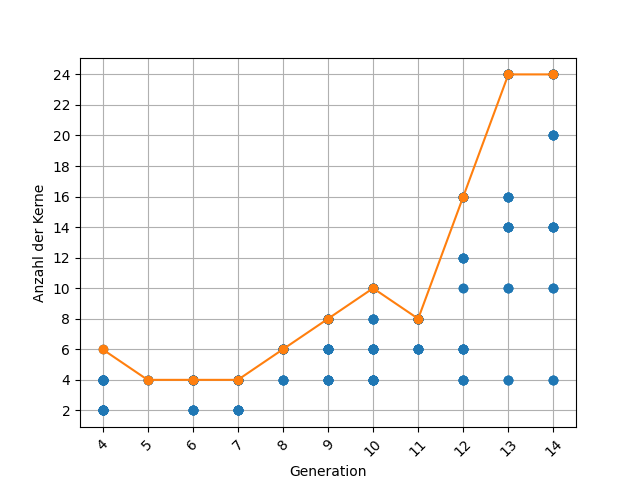
\includegraphics[width=0.49\textwidth]{Abbildung_1.png}
\label{fig:Abbildung_1}
\end{figure}

\begin{figure}[ht]
\hspace{-0.6cm}
\caption{\textbf{Anzahl der Kerne der X-series pro Prozessor-Generation von Intel} (Datenquelle: \cite{Comparison})}
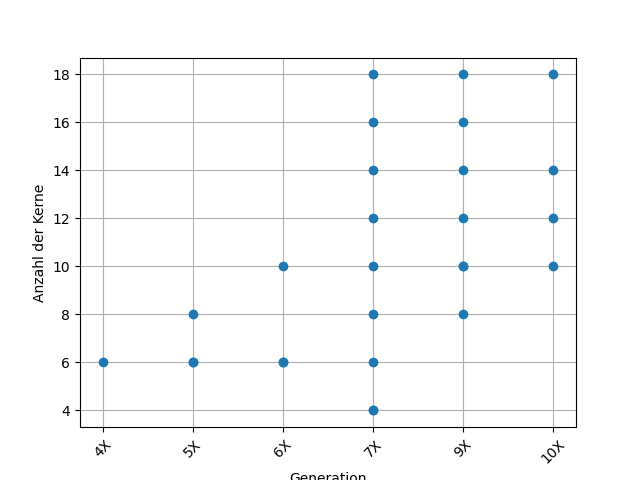
\includegraphics[width=0.49\textwidth]{Abbildung_2.png}
\label{fig:Abbildung_2} 
\end{figure}


\setlength{\parindent}{0pt}
    In Abbildung \ref{fig:Abbildung_1} und Abbildung \ref{fig:Abbildung_2} ist zu erkennen, 
    dass seit der Einführung der 4th Generation (Haswell) im Jahr 2013 \cite{intel-4th-gen-core} sich die Anzahl der Kerne bei Intel, 
    für Desktop Computer, von 6 auf 24 Kernen erhöht hat. 
    Es ist wichtig zu beachten, dass es zwar Prozessoren mit einer noch höheren Anzahl von Kernen gibt, 
    diese jedoch in der Regel für Server bestimmt sind.
    In der Abbildung \ref{fig:Abbildung_last} ist jedoch zu erkennen, dass die Gigahertz-Werte stagnieren.
\begin{figure}[ht]
\hspace{-0.6cm}
\caption{\textbf{Vergleich der Entwicklung der Speicherbandbreite und max. Rechenleistung} (Datenquellen: \cite{prozessoren})}
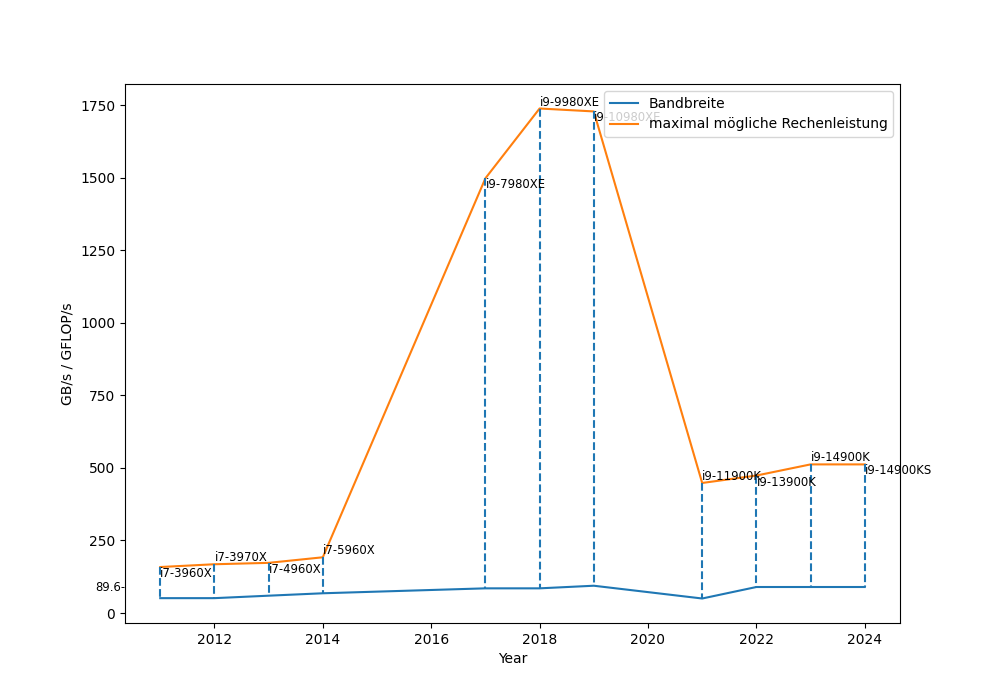
\includegraphics[width=0.49\textwidth]{Abbildung_3.png}
\label{fig:Abbildung_3}
\end{figure}
    Wenn man nun die theoretische maximale Rechenleistung, 
    definiert als:\\ $\textnormal{P}_{\textnormal{max}} = \textnormal{Anzahl der Kerne } \times \textnormal{ Turbo Taktfrequenz } \times \\\textnormal{ Flops pro Taktzyklus } \times \textnormal{ Anzahl der Instruktionssets}$,\\und
    der Entwicklung der Speicherbandbreite gegenüberstellt, wird in Abbildung \ref{fig:Abbildung_3} deutlich, 
    dass die Zunahme der Speicherbandbreite nicht im gleichen Maße wie die Rechenleistung ansteigt. 
    Im Detail hat sich die Bandbreite von dem i7-3960X von 51.2 $\frac{\text{GByte}}{\text{s}}$ im Jahr 2013 auf 89.6 $\frac{\text{GByte}}{\text{s}}$ bei dem i9-14900KS im Jahr 2024 erhöht. 
    Parallel dazu hat sich die theoretische maximale Rechenleistung im gleichen Zeitraum von 158.4 $\frac{\text{Flops}}{\text{s}}$ auf 512 $\frac{\text{Flops}}{\text{s}}$ gestiegen.
    In Abbildung \ref{fig:Abbildung_3} ist ein Flop definiert als eine Gleitkommazahl-Operation mit einer FP32-Zahl.
    Die Werte für die drei Prozessoren i9-7980XE, 
    i9-9980XE und i9-10980XE scheinen inkonsistent mit dem erwarteten Entwicklungstrend zu sein.
    Der Grund dafür ist, 
    dass diese drei Prozessoren über zwei 512-Bit-Instruktionssets verfügen. 
    Dies erhöht das Ergebnis der maximalen Rechenleistung erheblich im Vergleich zu den anderen Prozessoren, 
    die lediglich über ein AVX2 256-Bit-Instruktionsset verfügen.
    Diese Diskrepanz zwischen der gesteigerten Rechenleistung und der vergleichsweise langsamer wachsenden Speicherbandbreite 
    verdeutlicht die Notwendigkeit einer Optimierung von Datenzugriffen. 
    Ein effizienter Einsatz des Caches ist dabei unerlässlich, um die Leistung zu maximieren.
    Des Weiteren arbeitet der Intel® AMX, 
    eine spezielle Hardware-Komponente in Intel® Xeon® Scalable Prozessorkernen, 
    daran, 
    Matrix-Mathematik-basierte Deep-Learning-Workloads zu optimieren und zu beschleunigen. 
    Es erreicht dies, indem es mehr Daten pro Kern speichert und größere Matrizen in einer einzigen Operation berechnet, 
    ohne die Notwendigkeit, Workloads auf einen separaten Beschleuniger auszulagern \cite{TMUL}.

    \section{Die Berechnung der Performancegrenzen}
    In den nachfolgenden Unterabschnitten werden die Formeln vorgestellt, 
    die zur Bewertung von loop-basiertem Code und zur Berechnung der Performancegrenzen herangezogen werden. 
    Es ist jedoch wichtig zu berücksichtigen, dass diese Formeln lediglich eine Annäherung darstellen 
    und nur unter bestimmten Bedingungen gültig sind. Beispielsweise wird vorausgesetzt, 
    dass alle Ressourcen vollständig ausgeschöpft werden die die CPU zu bieten hat. 
    Zudem basieren die Formeln auf Aspekten des idealen Cache-Modells, 
    wie einem unendlich schnellen Cache und der Nichtexistenz von Latenzzeiten.

    \subsection{Maschinenbalance}

    Die Maschinenbalance $\textnormal{B}_{\textnormal{m}}$ ist das Verhältnis 
    aus der maximalen Bandbreite und der theoretischen Rechenleistung
    $\textnormal{B}_{\textnormal{m}} = \frac{\textnormal{B}_{\textnormal{max}}}{\textnormal{P}_{\textnormal{max}}}$.
    Sie beschreibt, wie viele Daten pro Flop übertragen werden können. Zur Veranschaulichung 
    betrachten wir die $\textnormal{B}_{\textnormal{m}}$ für den i7-9700K Prozessor,     % Hier muss ein Quellenverweis hin
    der 2018 erschienen ist und eine maximale Bandbreite von 41.6\,$\frac{\text{GByte}}{\text{s}}$ sowie
    eine theoretische Rechenleistung von 8\,Kerne $\times$ 4.9\,GHz $\times$ 16\,$\frac{\text{Flops}}{\text{Taktzyklus}}$ = 627,2\,$\frac{\text{Flops}}{\text{s}}$ besitzt.
    Die Bandbreite muss noch in Fließkommazahlen umgerechnet werden, die pro Sekunde geladen werden können. Also
    $\frac{41.6 \, \text{GB/s}}{8 \, \text{Byte}} = 5.2 \, \frac{\text{Fließkommazahlen}}{\text{s}}$.
    Daraus ergibt sich, dass $\textnormal{B}_{\textnormal{m}} = \frac{5.2 \, \textnormal{Fließkommazahlen/s}}{627.2 \, \textnormal{Flops/s}} \approx 0.008\,\frac{\textnormal{Fließkommazahlen}}{\textnormal{Flop}}$
    geladen werden können. Mit anderen Worten, bis eine Fließkommazahl geladen ist, müssen
    125 Flops auf einem Wert durchgeführt werden, bis der nächste Wert geladen ist. 
    Die Maschinenbalance bei den neuesten Prozessoren wie dem i9-14900KS liegt bei $\approx 0.0058$, und somit wären 
    172 Flops pro geladene Fließkommazahl erforderlich. Man könnte daher schlussfolgern, 
    dass das Rechnen quasi kostenlos ist und das Laden der Werte den limitierende Faktor darstellt.

    \subsection{Codebalance}
    Die Codebalance $\textnormal{B}_{\textnormal{c}} = \frac{\textnormal{Datenverkehr}}{\textnormal{Flops}}$ ist das Verhältnis
    der zu ladenden und speichernden Fließkommazahlen und der Anzahl der Flops in einer loop Iteration. 
    Hierbei zählt man aber nur die load und store Operationen, welche wirklich über den langsamen Datenpfad verläuft, daher wird $\text{l\_i}$ nicht mitgezählt,
    weil es sich im Register befindet.
    In Abbildung 4 ist ein solcher loop dargestellt, % Hier muss ein Quellenverweis hin
    welcher 4 Flops ausführt und 3 Elemente aus den drei Arrays $\textnormal{X}$, $\textnormal{Y}$ und $\textnormal{Z}$ lädt 
    und eine speicher Operation in $\textnormal{Z}$ durchführt. Die Codebalance ist also $\textnormal{B}_{\textnormal{c}} = \frac{3+1}{4} = 1$. 


    \subsection{Berechnung der zu erwartenden Performance}
    Um die maximal erreichbare Performance eines loop-basierten Codes zu berechnen, 
    bestimmt man den Anteil der maximalen CPU-Performance, die tatsächlich erreicht werden kann. 
    Dieser Anteil wird als ,,lightspeed" $\text{l}$ bezeichnet und ist definiert als 
    $\text{l} = \min(1, \frac{\text{B}_{m}}{\text{B}_{c}})$. 
    Da diese Formel auf den ersten Blick nicht intuitiv ist, 
    kann ein Beispiel zur Veranschaulichung dienen. 
    Betrachten wir erneut den Code aus Abbildung 4. 
    Die Maschinenbalance $\textnormal{B}_{\textnormal{m}}$ 
    beträgt 0.5 $\frac{\textnormal{Fließkommazahlen}}{\textnormal{Flop}}$, 
    während die Codebalance $\textnormal{B}_{\textnormal{c}}$ 1 beträgt, 
    da vier Fließkommazahlen geladen und gespeichert werden müssen und vier Flops ausgeführt werden. 
    Da das Bereitstellen und Abspeichern von Fließkommazahlen nicht so schnell ist wie das Rechnen 
    (was durch $\textnormal{B}_{\textnormal{m}}$  = 0.5 ausgedrückt wird), kann man in der Zeit, 
    in der man vier Flops ausführen würde, 
    nur halb so viele, also 4 $\times$ 0.5 = 2 Fließkommazahlen laden und/oder abspeichern.
    Daher ist die maximale Performance, die erreicht werden kann, 
    $\text{l} = \min(1, \frac{0.5}{1}) = 0.5$. 
    
    Oder anders betrachtet, es könnte einen Code geben,
    der doppelt so viele Flops ausführt wie er Fließkommazahlen lädt und speichert. 
    Dies würde zu einer Codebalance von 0.5 führen. 
    In einem solchen Szenario wäre die Anzahl 
    der zu ladenden und speichernden Fließkommazahlen genau gleich der theoretisch möglichen Anzahl
    an Fließkommazahlen, die geladen und gespeichert werden könnten. 
    Somit würde der maximal zu erreichende Anteil an 
    $\textnormal{P}_{\textnormal{max}}$ bei $\text{l} = \min(1, \frac{0.5}{0.5}) = 1$ liegen.  % Hier muss ein Quellenverweis hin
    Wenn dieser Wert nah an 1 liegt ist man nicht Speichergebunden.
    Die maximal erreichbare Performance ist somit $\textnormal{P} =  \textnormal{l} \times \textnormal{P}_{\textnormal{max}}$ oder 
    $\textnormal{P} =  \min(\textnormal{P}_{\textnormal{max}}, \frac{\textnormal{b}_{\textnormal{max}}}{\textnormal{B}_{\textnormal{c}}})$.

\section{Loop Fusion} 
    Die erste Methode, die zur Optimierung des Zugriffsverhaltens vorgestellt 
    wird und bei der anhand des präsentierten Modells eine Verbesserung erkennbar ist, 
    ist Loop Fusion. Es ist wichtig zu verstehen, dass der Cache ein kleiner, 
    schneller Speicher ist, der die Least Recent Used (LRU) Policy verwendet, um zu entscheiden, 
    welche Daten im Cache verbleiben. Dies bedeutet, 
    dass die am längsten nicht genutzten Daten aus dem Cache entfernt werden, 
    wenn eine neue Cache Line geladen werden muss und kein Platz mehr im Cache vorhanden ist. 
    Dies beschreibt die zeitliche Lokalität. 
    Wenn eine Cache Line geladen wird und die umliegenden Daten ebenfalls in den Cache geladen werden, 
    spricht man von räumlicher Lokalität, da man davon ausgeht, 
    dass diese Daten in naher Zukunft ebenfalls genutzt werden. 
    Typischerweise beträgt die Größe einer Cache-Zeile 64 Bytes, 
    kann aber durch die Befehle \texttt{getconf LEVEL1\_DCACHE\_LINESIZE}, 
    \texttt{getconf LEVEL2\_CACHE\_LINESIZE},
    \texttt{getconf LEVEL3\_CACHE\_LINESIZE} 
    leicht bestimmt werden. Um die Größe des Caches zu ermitteln, 
    kann man den Befehl \texttt{lstopo} verwenden, sofern installiert. 
    Betrachtet man Abbildung 5, ist % hier muss ein Quellenverweis hin
    leicht zu erkennen, dass zunächst in einer for-Schleife die Elemente aus dem Array 
    $\textnormal{A}$ mit dem Skalar $\textnormal{2.0}$ 
    multipliziert und in das Array $\textnormal{Z}$ gespeichert werden. 
    Anschließend wird eine weitere for-Schleife ausgeführt, die das Gleiche tut, 
    nur dass hier das Ergebnis in $\textnormal{Y}$ gespeichert wird. 
    Wenn die Arrays zu groß sind und am Ende der ersten for-Schleife die Cache Line, 
    die die ersten Elemente aus A enthält verdrängt wurde, 
    müssen diese für die zweite for-Schleife erneut in den Cache geladen werden. 
    Daten, die in den Cache geladen und aus Platzgründen wieder verdrängt wurden, 
    aber später wieder benötigt und erneut in den Cache geladen werden, nennt man 
    \texttt{Capacity Miss}. Das erstmalige Laden von Daten über langsame Datenpfade wird als 
    \texttt{Cold Miss} bezeichnet. Die Code-Balance $\textnormal{B}_{\textnormal{c}}$ 
    der beiden for-Schleifen beträgt $\frac{2}{1} = 2$. Wenn man jedoch die beiden 
    for-Schleifen zusammenführt (siehe Abbildung 6), spart man sich einen langsamen Load, % hier muss ein Quellenverweis hin
    da der Wert von A[i] in der Zeile zuvor in den Cache geladen wurde, 
    wodurch sich die Code-Balance auf $\frac{3}{2} = 1.5$ reduziert. 
    Um das Modell zu überprüfen, wurden beide Varianten gebenchmarkt. 
    Die Ergebnisse sind in Abbildung 7 dargestellt. Man erkennt, % hier muss ein Quellenverweis hin
    dass die Loop-Fusion-Variante schneller ist als die nicht fusionierte Variante.

\section{Der STREAM Benchmark}
    Der STREAM Benchmark besteht aus vier Kernels, die die Bandbreite des Speicherinterfaces meist in GB/s messen sollen.
    Die vier Kernels sind Copy, Scale, Add und Triad wobei in der Tabelle auch die Codebalance nochmal aufgeführt ist.
    

    \begin{table}[h]
        \centering
        \begin{tabular}{|c|c|c|c|}
        \hline
        \textbf{Kernelname} & \textbf{Operation} & \textbf{Code-Balance} \\
        \hline
        Copy & A[i] = B[i] & - \\
        \hline
        Scale & A[i] = q*B[i] & 2/1 \\
        \hline
        Add & A[i] = B[i] + C[i] & 2/1 \\
        \hline
        Triad & A[i] = B[i] + q*C[i] & 3/2 \\
        \hline
        \end{tabular}
        \caption{STREAM Benchmark Kernels und ihre Code-Balance}
        \label{tab:stream_benchmark}
        \end{table}


    Für die Ausführung des STREAM-Benchmarks ist es wichtig, 
    dass die Datenmengen ausreichend groß sind. AMD empfiehlt, 
    dass die Arrays mindestens viermal so groß sein sollten wie die Summe aller Last-Level-Caches. % Hier muss ein Quellenverweis hin. 
    Im vorherigen Abschnitt wurde der Scale-Kernel genutzt, 
    um die Effektivität der Loop-Fusion zu demonstrieren. 
    Dabei wurde die Zeit jedoch in Nanosekunden anstelle von GB/s gemessen. 
    Da diese synthetischen Kernels die Hardware direkt testen, 
    sind die erreichten Bandbreitenwerte aussagekräftigere Vergleichswerte als die, 
    die man beispielsweise auf den Webseiten von AMD oder Intel findet, 
    um die Leistung von Code und Hardware einzuschätzen. % Hier muss ein Quellenverweis hin.
    Abbildung 8 stellt die Ergebnisse des Triad-Kernels auf einem i7-9700K dar. % Hier muss ein Quellenverweis hin. 
    Es ist erkennbar, dass die Bandbreite mit jedem Cache-Level abnimmt, 
    wobei der Rückgang bei dem L3-Cache besonders stark ist. 
    Derselbe Benchmark wurde auch auf dem ARA-Cluster auf einem der FSU Jena durchgeführt. 
    Die Ergebnisse, die in Abbildung 9 dargestellt sind, verdeutlichen nochmals, 
    wie die Bandbreite von Cache-Level zu Cache-Level abnimmt. % Hier muss ein Quellenverweis hin.
    Sind Ergebnisse eines passenden Tests vorhanden sollte man also die vorhin vorgestellte Formel zur Berechnung der maximalen erreichbaren
    Performance zu $\textnormal{P} =  \min(\textnormal{P}_{\textnormal{max}}, 
    \frac{\textnormal{b}_{\textnormal{Stream}}}{\textnormal{B}_{\textnormal{c}}})$ abändern.

\section{Die Optimierung des Speicherzugriffsmusters}
    In Computern werden Daten linear im Speicher abgelegt, das heißt, sie werden in einer sequenziellen Reihenfolge gespeichert, 
    wobei zum Beispiel ein Byte eine eindeutige Adresse hat, die auf den genauen Speicherort verweist. Diese lineare Anordnung ermöglicht es, 
    effizient auf Daten zuzugreifen, 
    indem man die Adresse des gewünschten Datenstücks kennt oder berechnet.
    Greift man auf ein Element zu, dann wird die zugehörige Cache Line geladen, wenn die Cache Line sich noch nicht im Cache befindet.
    Im besten Fall werden anschließend alle Elemente der Cache Line abgerufen dann die Cache Line verdrängt 
    und nie wieder benötigt. Im schlechtesten Fall wird die Cache Line verdrängt bevor alle Elemente abgerufen wurden 
    oder sogar nur ein Element genutzt, wodurch der Zweck des Caches verfehlt wird.
    In Abbildung 10 ist ein Beispiel für ein 2D Array in Row-Major-Order dargestellt. % Hier muss ein Quellenverweis!!!!! hin.
    Würde man in dieser Matrix Spaltenweise auf die Elemente zugreifen,
    dann würde jeder Zugriff das Laden einer neuen Cache Line erfordern, 
    weil man restlichen Elemente der Zeile überspringt.
    Die Schrittweite von einem Zugriff nennt man Stride.
    Überspringt man beispielsweise n Elemente, dann dann ist das ein Stride von n Elementen.
    Um die Auswirkungen des Speicherzugriffsmusters zu demonstrieren, sind hier (\hyperref[fig:Zeilenorientierte Matrix Matrix Multiplikation]{klicke hier}) zwei C++ 
    Varianten einer Matrix Matrix Multiplikation dargestellt. Die Elemente der Matrizen sind 
    in Row Major abgespeichert und die Matrizen sind quadratisch und gleich groß.


\begin{tiny}
    \begin{adjustwidth}{-0,37cm}{}
    \begin{footnotesize}
    \begin{auflistung}
    \caption{Zeilenorientierte Matrix Matrix Multiplikation}
    \label{fig:Zeilenorientierte Matrix Matrix Multiplikation}
    \begin{minted}[linenos, gobble=2,xleftmargin=-0.3cm, numbersep=-12pt]{cpp}
        void gemm_mkn(double* X, double* Y, double* Z, std::size_t n){
    
        for (std::size_t l_m = 0; l_m < n; l_m++)
        {
            for (std::size_t l_k = 0; l_k < n; l_k++)
            {
                for (std::size_t l_n = 0; l_n < n; l_n++)
                {
                   Z[l_m * n + l_n] += X[l_m * n + l_k] * Y[l_k * n + l_n];
                }
            }
        }
        }
        
    \end{minted}
    \end{auflistung}
    Die Elemente von Z, X und Y werden für die Matrix Matrix Multiplikation mit einem \\
    \hspace*{0.36cm}Stride-N-Muster abgerufen.
    \end{footnotesize}
    \end{adjustwidth}
    \end{tiny}


    \label{fig:Spaltenorientierte Matrix Matrix Multiplikation}
\begin{tiny}
    \begin{adjustwidth}{-0,37cm}{}
    \begin{footnotesize}
    \begin{auflistung}
    \caption{Zeilenorientierte Matrix Matrix Multiplikation}
    \begin{minted}[linenos, gobble=2,xleftmargin=-0.3cm, numbersep=-12pt]{cpp}
        void gemm_nkm(double* X, double* Y, double* Z, std::size_t n){

        for (std::size_t l_n = 0; l_n < n; l_n++)
        {
            for (std::size_t l_k = 0; l_k < n; l_k++)
            {
                for (std::size_t l_m = 0; l_m < n; l_m++)
                {
                   Z[l_m * n+ l_n] += X[l_m * n + l_k] * Y[l_k * n + l_n];
                }
            }
        }
        }
    \end{minted}
    \end{auflistung}
    Die Elemente von Z, X und Y werden für die Matrix Matrix Multiplikation mit einem \\
    \hspace*{0.36cm}Stride-N-Muster abgerufen.
    \end{footnotesize}
    \end{adjustwidth}
    \end{tiny}



\,\\Um zu entscheiden welcher der beiden Implementierungen effizienter ist,
ohne sie zu benchmarken kann man sich jeweils die Zugriffsmuster ansehen.
In der ersten Implementierung wird auf die Elemente von Z mit einem $\textnormal{Stride-1}$ zugegriffen,
dabei wird die selbe Zeile n-Mal durchlaufen bis die nächste Zeile bearbeitet wird.
Auf das gleiche Element von X wird n-Mal zugegriffen, bevor mit einem Stride-1 auf das nächste Element zugegriffen wird.
Dabei bleibt man bei X auch in der selben Zeile, also in der selben Cache Line.
Bei Y wird sich zeilenweise durch die Matrix gearbeitet und dies n-Mal wiederholt. Die Abbildung \ref{fig:Visualisierung der ersten Implementierung}
zeigt nochmal das Verhalten des Algorithmus.
Es ist wichtig zu beachten, dass eine Cache Line deutlich kleiner ist als eine Zeile/Spalte und dass dies lediglich ein Modell darstellt, 
keine direkte Abbildung einer Matrix-Matrix-Multiplikation.\\
\textbf{Abbildung 5: Visualisierung der ersten Implementierung}
\label{fig:Visualisierung der ersten Implementierung}

\begin{tikzpicture}[scale=0.28]
    % Matrix C
    \draw (0,0) rectangle (7,7);
    \foreach \i in {1,...,6} {
        \draw (\i,0) -- (\i,7);
        \draw (0,\i) -- (7,\i);
    }
    \foreach \i in {0,...,6} {
        \fill[red, opacity=0.3] (\i,6) rectangle (\i+1,7);
    }
    \node at (3.5,-0.5) {Z};

    % Loop symbol for Matrix C
    \draw[->] (0.5,6.5) to[bend left=30] (6.5,6.5) to[bend left=10] (0.3,6.5);
    \node at (3.5,8) {n-Mal};

    % += symbol
    \node at (8.5,3.5) {+=};

    % Matrix A
    \draw (10,0) rectangle (17,7);
    \foreach \i in {1,...,6} {
        \draw (10+\i,0) -- (10+\i,7);
        \draw (10,\i) -- (17,\i);
    }

    % Fill the first row with red color
    \foreach \i in {0,...,6} {
        \fill[red, opacity=0.3] (10+\i,6) rectangle (11+\i,7);
    }

    % Loop symbol for the first row of Matrix A
    \foreach \i in {0,...,6} {
        \draw[->] (10.5+\i,6.5) to[bend left=80] (10.5+\i,7.5) to[bend left=0] (10.5+\i,6.5);
    }
    \node at (13.5,8) {n-Mal jeweils};

    % Matrix name
    \node at (13.5,-0.5) {X};

    % * symbol
    \node at (18.5,3.5) {*};

    % Matrix B
    \draw (20,0) rectangle (27,7);
    \foreach \i in {1,...,6} {
        \draw (20+\i,0) -- (20+\i,7);
        \draw (20,\i) -- (27,\i);
    }
    \foreach \i in {0,...,6} {
        \foreach \j in {0,...,6} {
            \fill[red, opacity=0.3] (20+\i,6-\j) rectangle (21+\i,7-\j);
        }
    }
    % Matrix name
    \node at (23.5,-0.5) {Y};

    % Zigzag line with arrow
    \node at (23.5,-0.5) {Y};
    \draw[->] (20.5,6.5) -- (26.5,6.5) -- (20.5,5.5) -- (26.5,5.5) -- (20.5,4.5) -- (26.5,4.5) -- (20.5,3.5) -- (26.5,3.5) -- (20.5,2.5) -- (26.5,2.5) -- (20.5,1.5) -- (26.5,1.5) -- (20.5,0.5) -- (26.5,0.5);
    \node at (29,3.5) {n-Mal};

\end{tikzpicture}


In der zweiten Implementierung \ref{fig:Spaltenorientierte Matrix Matrix Multiplikation} wird immer die Zeile übersprungen, 
wenn ein neues Element geladen wird. Dies führt dazu, 
dass die zweite Implementierung bei jedem neuen Element eine neue Cache Line laden muss. 
In Abbildung \ref{fig:Visualisierung der zweiten Implementierung} ist das Verhalten der zweiten Implementierung dargestellt.
Es ist wichtig zu beachten, dass eine Cache Line deutlich kleiner ist als eine Zeile/Spalte und dass dies lediglich ein Modell darstellt, 
keine direkte Abbildung einer Matrix-Matrix-Multiplikation.
\textbf{Abbildung 12: Visualisierung der zweiten Implementierung}


\label{fig:Visualisierung der zweiten Implementierung}
\begin{adjustbox}{left}
    \begin{tikzpicture}[scale=0.275, >={Stealth[length=10pt, width=3pt]}]
        % Matrix Z
        \draw (0,0) rectangle (7,7);
        \foreach \i in {1,...,6} {
            \draw (\i,0) -- (\i,7);
            \draw (0,\i) -- (7,\i);
        }
        \foreach \i in {0,...,6} {
            \fill[red, opacity=0.3] (0,\i) rectangle (1,\i+1);
        }
        \node at (3.5,-0.5) {Z};
    
        % Loop symbol for Matrix Z
        \draw[->] (0.5,6.5) to[bend right=30] (0.5,0.5) to[bend right=10] (0.5,6.3);
        \node at (-2,3.5) {n-Mal};
    
        % += symbol
        \node at (8.5,3.5) {+=};
    
        % Matrix X
        \draw (10,0) rectangle (17,7);
        \foreach \i in {1,...,6} {
            \draw (10+\i,0) -- (10+\i,7);
            \draw (10,\i) -- (17,\i);
        }
    
        % Fill all elements with red color
        \foreach \i in {0,...,6} {
            \foreach \j in {0,...,6} {
                \fill[red, opacity=0.3] (10+\i,\j) rectangle (11+\i,\j+1);
            }
        }
    
        % Zigzag line with arrow for Matrix X
        \foreach \i in {0,...,5} {
            \draw (10.5+\i,6.5) -- (10.5+\i,0.5) -- (11.5+\i,6.5);
        }
        \draw (15.5,6.5) -- (15.5,0.5) -- (16.5,6.5);
        \draw[->] (16.5,6.5) -- (16.5,0.5);
        \node at (13.5,8) {n-Mal};
    
        % Matrix name
        \node at (13.5,-0.5) {X};
    
        % * symbol
        \node at (18.5,3.5) {*};
    
        % Matrix Y
        \draw (20,0) rectangle (27,7);
        \foreach \i in {1,...,6} {
            \draw (20+\i,0) -- (20+\i,7);
            \draw (20,\i) -- (27,\i);
        }
        \foreach \i in {0,...,6} {
            \fill[red, opacity=0.3] (20,6-\i) rectangle (21,7-\i);
        }
        % Matrix name
        \node at (23.5,-0.5) {Y};
        \node at (20.5,8) {n-Mal jeweils};
    
        % Loop symbol for the first column of Matrix Y
        \foreach \i in {0,...,6} {
            \draw[->] (20.5,6.5-\i) to[bend right=80] (19.5,6.5-\i) to[bend right=0] (20.5,6.5-\i);
        }
        
        \end{tikzpicture}
        \end{adjustbox}


Bei ausreichend großen Matrizen kommt es zu ständigen Capacity Misses. 
Die Anzahl dieser kann einfach approximiert werden, 
indem man den einfachen Fall betrachtet, 
dass jeweils eine Zeile oder Spalte für Z, X und Y im Cache gehalten werden kann.
Es gibt $ \frac{\textnormal{n} \times \textnormal{n}}{\textnormal{L}} $ Cache Lines. 
Das erstmalige Laden jeder Cache Line für Z ist ein Cold Miss, 
aber die restlichen Zugriffe auf die gleiche Cache Line sind Capacity Misses. 
Das bedeutet, es gibt $\textnormal{n} * \textnormal{n} * \textnormal{n} - \frac{\textnormal{n} \times \textnormal{n}}{\textnormal{L}} $ 
Capacity Misses bei Z, wobei L die Anzahl der Elemente 
in einer Cache Line ist.
Bei X ist es ein ähnlicher Fall, da auch jedes Element nach einmaliger Nutzung in naher Zukunft verdrängt wird 
und später wieder benötigt wird. 
Es gibt also ebenfalls 
$\textnormal{n} * \textnormal{n} * \textnormal{n} - \frac{\textnormal{n} \times \textnormal{n}}{\textnormal{L}} $ 
Capacity Misses bei X.
Bei Y wird jedes Element n-Mal genutzt, bevor die Cache Line verdrängt wird. 
Daher kann man nur für jedes Element einen Capacity Miss zählen, 
mit Ausnahme des ersten Elemente jeder Cache Line. Anders ausgedrückt, 
es gibt $\textnormal{L} - 1 $ Capacity Misses pro Cache Line. 
Da es $ \frac{n \times \textnormal{n}}{\textnormal{L}} $ Cache Lines gibt, 
sind insgesamt $ \frac{\textnormal{n} \times \textnormal{n}}{\textnormal{L}} \times (\textnormal{L} - 1) $ Capacity Misses bei Y zu verzeichnen.
Insgesamt ergeben sich also 
$2 * \textnormal{n} * \textnormal{n} * \textnormal{n} - \frac{\textnormal{n} \times \textnormal{n}}{\textnormal{L}} + \frac{\textnormal{n} \times \textnormal{n}}{\textnormal{L}} \times (\textnormal{L} - 1) $ Capacity Misses.
Bei der ersten Implementierung hingegen gibt es keine Capacity Misses bei Z, 
da man stets eine Zeile für Z im Cache halten kann, ebenso wie bei X. 
Bei Y durchläuft man die Matrix zwar auch in Row-Major-Order, 
jedoch wird die erste Zeile nach der Bearbeitung der letzten verdrängt sein.
In der ersten Implementierung iteriert man n-Mal durch die Matrix Y. 
Der erste Durchlauf führt ausschließlich zu Cold Misses, 
während in den folgenden Durchläufen lediglich das erste Element jeder Cache Line einen Capacity Miss verursacht. 
Daher ergibt sich eine Gesamtzahl von $(\textnormal{n}-1) \times \frac{\textnormal{n} \times \textnormal{n}}{\textnormal{L}} $ Capacity Misses. 
Da die Anzahl der Capacity Misses bei der zweiten Implementierung deutlich höher ist, 
wird erwartet, dass die erste Implementierung, 
insbesondere bei großen Werten von \texttt{n}, eine bessere Performance aufweist.
In den Abbildungen \ref{Performance der verschiedenen Implementierungen der Matrix-Matrix Multiplikation} ist die Performance der beiden Implementierungen und die 4 restlichen 
Möglichkeiten der Matrix-Matrix Multiplikation dargestellt.\\\\ % Hier muss ein Quelle hin!!


\begin{figure}[ht]
    \centering
    \caption{Bandbreitenergebnisse der verschiedenen Implementierungen der Matrix-Matrix Multiplikation}
    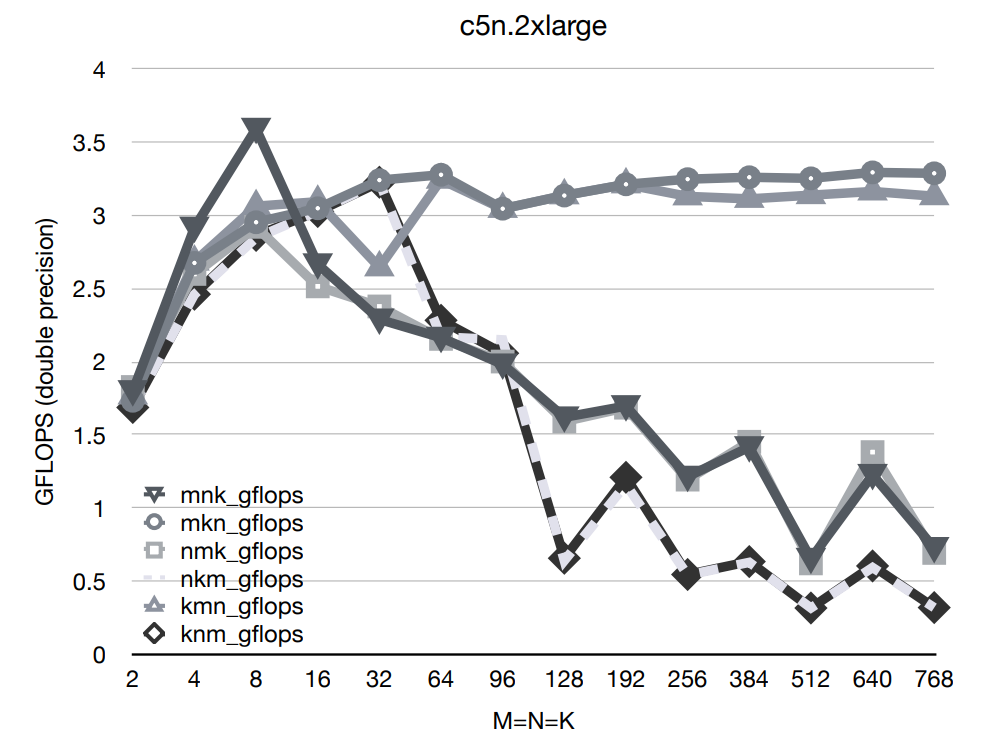
\includegraphics[width=0.4\textwidth]{Abbildung 13.png}
    \label{Performance der verschiedenen Implementierungen der Matrix-Matrix Multiplikation}
    \end{figure}
(Quelle : \cite{Breuer_Benchmark_PC1})

Die zeitlichen Werte für die beiden vorgestellten Implementierungen \ref{fig:Zeilenorientierte Matrix Matrix Multiplikation} und \ref{fig:Spaltenorientierte Matrix Matrix Multiplikation}, 
die auf dem i7-9700K Prozessor erzielt wurden, sind in Abbildung \ref{Performance der beiden Implementierungen der Matrix-Matrix Multiplikation} dargestellt.

\begin{figure}[ht]
    \centering
    \caption{Zeitliche Ergebnisse der verschiedenen Implementierungen der Matrix-Matrix Multiplikation}
    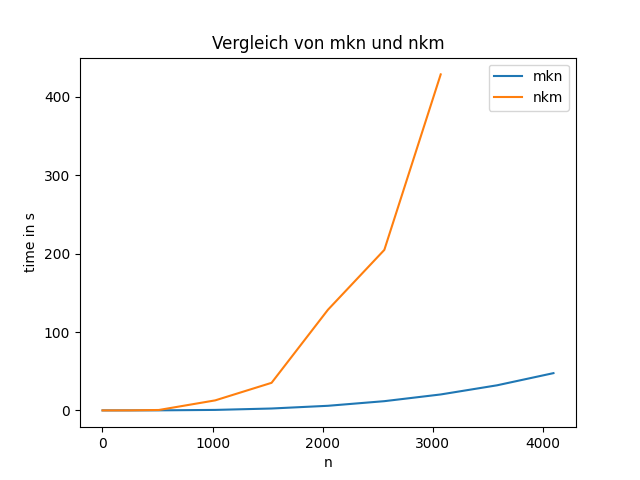
\includegraphics[width=0.4\textwidth]{Abbildung 14.png}
    \label{Performance der beiden Implementierungen der Matrix-Matrix Multiplikation}
    \end{figure}
In beiden Abbildungen ist zu erkennen das die Analyse der Zugriffsmuster und die Berechnung der Capacity Misses
einen guten Hinweis darauf geben können welcher Code effizienter arbeitet und das das Zugriffsmuster starken
Einfluss auf die Leistung hat.



\section{Unroll and Jam}
\begin{figure}[ht]
    \centering
    \caption{Zugriffsmuster von einer Matrix Vektor Multiplikation \cite{hager-2010}}
    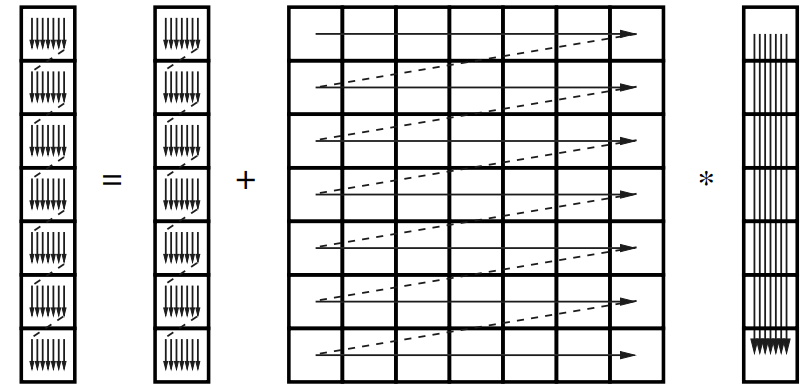
\includegraphics[width=0.4\textwidth]{Abbildung 16.png}
    \label{MVM Zugriffsmuster}
    \end{figure}

    \begin{tiny}
        \begin{adjustwidth}{-0,37cm}{}
        \begin{footnotesize}
        \begin{auflistung}
        \caption{Zeilenorientierte Matrix Matrix Multiplikation}
        \label{MVM Code}
        \begin{minted}[linenos, gobble=2,xleftmargin=-0.3cm, numbersep=-12pt]{cpp}
            void MVM(double* A, double* B, double* C, std::size_t n){

                for (std::size_t l_i = 0; l_i < n; l_i++)
                {
                    for (std::size_t l_j = 0; l_j < n; l_j++)
                    {
                        C[l_i] += A[l_i * n + l_j] * B[l_j]; 
                    }
                }
            }
            
        \end{minted}
        \end{auflistung}
        \end{footnotesize}
        \end{adjustwidth}
        \end{tiny}

Gegeben ist eine unoptimierte Implementierung einer Matrix-Vektor-Multiplikation,
die in Abbildung \ref{MVM Zugriffsmuster} dargestellt ist und
analysieren den zugehörigen Code in Auflistung \ref{MVM Code}.
Jedes Element von C wird n-Mal wiederholt verwendet, bevor das nächste Element mit einem Stride-1 geladen wird.
Array A wid ein mal durchlaufen aber für jede äußere Schleifeniteration wird einmal durch das Array B iteriert.
Um die Anzahl der Ladevorgänge für B zu reduzieren, 
kann man die Technik Unroll and Jam anwenden.
Dabei wird die äußere Schleife nicht mehr um eins, 
sondern um \(m\) inkrementiert. 


In der inneren for-Schleife wird dann der Code \(m\)-mal repliziert.
Dies bedeutet, dass für jede Iteration der äußeren Schleife \(m\) 
Berechnungen gleichzeitig durchgeführt werden. Das Ergebnis 

\begin{tiny}
    \begin{adjustwidth}{-0,37cm}{}
    \begin{footnotesize}
    \begin{auflistung}
    \caption{Implementierung der Matrix-Vektor-Multiplikation mit Unroll and Jam}
    \label{MVM Code}
    \begin{minted}[linenos, gobble=2,xleftmargin=-0.3cm, numbersep=-12pt]{cpp}
        void MVM(double* A, double* B, double* C, std::size_t n, std::size_t l_m){

        for (std::size_t l_i = 0; l_i < n;l_i = l_i + l_m)
        {
            for (std::size_t l_j = 0; l_j < n; l_j++)
            {
                C[l_i] = C[l_i] + A[l_i * n + l_j] * B[l_j]
                C[l_i] = C[l_i+1] + A[(l_i+1) * n + l_j] * B[l_j]
                //! m times ...
                C[l_i + l_m-1] = C[i+m-1] + A[(l_i+m-1) * n + l_j] * B[l_j]
            }
        }

        }
        
    \end{minted}
    \end{auflistung}
    \end{footnotesize}
    \end{adjustwidth}
    \end{tiny}





Wir nehmen der Einfachheit halber an, dass $\textnormal{n}\%\textnormal{m} = 0$ und dass $\textnormal{m} = 0$ nicht zu groß gewählt wird.
All dies setzt jedoch voraus, 
dass der Registerdruck nicht zu groß ist, 
also dass die CPU genügend Register hat, 
um alle benötigten Operanden in dem nun größeren Schleifenkörper zu halten. Wenn dies nicht der Fall ist, muss der Compiler Registerdaten in den Cache auslagern, 
was die Berechnung verlangsamt.Hier können Compiler-Protokolle helfen, eine solche Situation zu identifizieren \cite{hager-2010v2}.
In Auflistung \ref{MVM Code} wird nun jedes Element von B \(m\)-mal verwendet in der inneren Schleife, bevor das nächste Element geladen wird.
Anders gesagt reduziert sich die Anzahl der Ladevorgänge für B von $\textnormal{n} \times \textnormal{n} $ auf $\frac{\textnormal{n} \times \textnormal{n}}{\textnormal{m}}$.



\section{Das Transponieren einer Matrix}
\begin{tiny}
    \begin{adjustwidth}{-0,37cm}{}
    \begin{footnotesize}
    \begin{auflistung}
    \caption{unoptimierte Version: Transponieren einer Matrix}
    \label{Transponieren einer Matrix}
    \begin{minted}[linenos, gobble=2,xleftmargin=-0.3cm, numbersep=-12pt]{cpp}
    void transpose(double* A, double* B, std::size_t n)
    {
        for (std::size_t l_y = 0; l_y < n; l_y++)
        {
            for (std::size_t l_x = 0; l_x < n; l_x++)
            {
                B[l_x * n + l_y] = A[l_y * n + l_x];
            }
        }
    }
        
    \end{minted}
    \end{auflistung}
    \end{footnotesize}
    \end{adjustwidth}
    \end{tiny}




Die intuitive Lösung zum Transponieren einer beispielsweise quadratischen Matrix ist in Auflistung \ref{Transponieren einer Matrix} dargestellt.
(Die Elemente sind in Row-Major-Order abgespeichert)

\,\\
Diese Implementierung durchläuft Matrix A zeilenweise und fügt Elemente spaltenweise in Matrix B ein,
was zu strided Store-Operationen führt. Diese sind in der Regel teurer als strided Load-Operationen,
da bei einem Cache-Miss die Cache-Zeile geladen und nach einer Änderung 
zurück in den langsameren Speicher geschrieben werden muss, statt sie einfach zu verwerfen.



\begin{tiny}
    \begin{adjustwidth}{-0,37cm}{}
    \begin{footnotesize}
    \begin{auflistung}
    \caption{strided load Version: Transponieren einer Matrix}
    \label{Transponieren einer Matrix strided load}
    \begin{minted}[linenos, gobble=2,xleftmargin=-0.3cm, numbersep=-12pt]{cpp}
    void transpose(double* A, double* B, std::size_t n)
    {
        for (std::size_t l_y = 0; l_y < n; l_y++)
        {
            for (std::size_t l_x = 0; l_x < n; l_x++)
            {
                B[l_y * n + l_x] = A[l_x * n + l_y];
            }
        }
    }
        
    \end{minted}
    \end{auflistung}
    \end{footnotesize}
    \end{adjustwidth}
    \end{tiny}


    \begin{figure}[h]
        \hspace{-0.46cm} % Passen Sie diesen Wert an, um das Bild zu verschieben
        \caption{Bandbreitenergebnisse}
        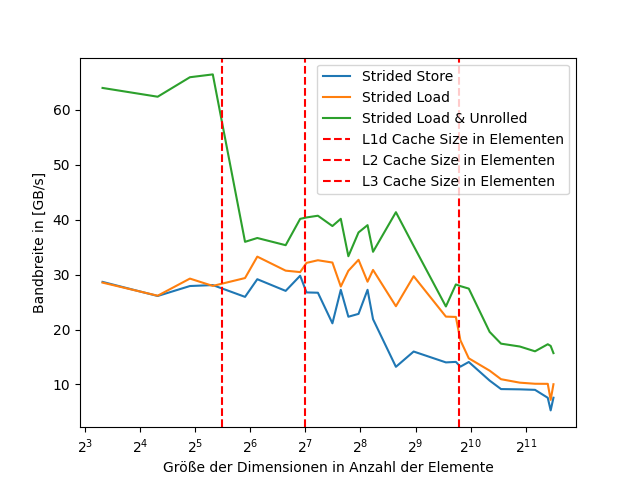
\includegraphics[width=0.46\textwidth]{Abbildung 15.png}
        \label{strided load vs. strided store}
    \end{figure}
Die erste Optimierung besteht darin, in Zeile 7 die Load-Operation strided zu wählen 
siehe Auflistung \ref{Transponieren einer Matrix strided load}.
Die Elemente von A werden nun spaltenweise geladen und in B zeilenweise gespeichert.
In der Abbildung \ref{strided load vs. strided store} ist der Vergleich der Implementierungen auf dem i7-9700K dargestellt und 
es ist zu erkennen, dass die strided Load Implementierung im Allgemeinen eine höhere Bandbreite aufweist.


Die effektive Bandbreite bei der Verarbeitung großer Datenmengen, 
die den L3-Cache überschreiten, beträgt etwa 10 GB/s. 
Ein Hauptproblem bei der Arbeit mit großen Dimensionen besteht darin, 
dass der Cache ständig überschrieben wird und Cachezeilen verdrängt werden, 
obwohl sie in naher Zukunft erneut benötigt werden könnten.

Bei großen Dimensionen führt das Stride-n Zugriffsmuster bei A häufig zu einem Cache-Miss, 
was das Laden einer neuen Cachezeile erfordert. 
Diese wird dann jedoch nur für ein einziges Element verwendet, 
was die Bandbreite bei großen Dimensionen erheblich reduziert.


\begin{tiny}
    \begin{adjustwidth}{-0,37cm}{}
    \begin{footnotesize}
    \begin{auflistung}
    \caption{Unroll und jam Version von: Transponierens einer Matrix}
    \label{UNROLLANDJAMVERSIONTRANSPONIERENMATRIX}
    \begin{minted}[linenos, gobble=2,xleftmargin=-0.3cm, numbersep=-12pt]{cpp}
    for (size_t l_j = 0; l_j < array_size; l_j = l_j + 5)
    {
    for (size_t l_i = 0; l_i < array_size; l_i++)
    {
        array_B[l_j * array_size + l_i] = 
        array_A[l_i * array_size + l_j];

        array_B[(l_j + 1) * array_size + l_i] = 
        array_A[l_i  * array_size + l_j + 1];

        array_B[(l_j + 2) * array_size + l_i] = 
        array_A[l_i  * array_size + l_j + 2];

        array_B[(l_j + 3) * array_size + l_i] = 
        array_A[l_i  * array_size + l_j + 3];
        
        array_B[(l_j + 4) * array_size + l_i] = 
        array_A[l_i  * array_size + l_j + 4];
    }
    }
    \end{minted}
    \end{auflistung}
    \end{footnotesize}
    \end{adjustwidth}
    \end{tiny}



Eine mögliche Strategie zur Optimierung der Cache-Nutzung besteht darin, 
mehr als ein Element pro Cachezeilen-Ladevorgang von A zu verwenden. 
Dies kann durch die zuvor vorgestellte Unroll-and-Jam-Technik erreicht werden. 
Bei dieser Technik werden bei jeder inneren Operation m Elemente gleichzeitig 
aus meist nur einer Cachezeile von A genutzt und in B gespeichert. 
Der Nachteil dabei ist, dass B ständig mindestens m Cachezeilen belegt hält. 
In der Auflistung \ref{UNROLLANDJAMVERSIONTRANSPONIERENMATRIX} wird eine 
Implementierung des Matrixtransponierens mit Unroll and Jam gezeigt, 
wobei hier m = 5 gewählt wurde. 
In der Abbildung \ref{strided load vs. strided store} ist zu erkennen, 
dass diese Implementierung eine höhere Bandbreite aufweist als die Strided-Load-Implementierung. 
Insbesondere wenn die Matrizen zusammen größer sind als der Last-Level-Cache, 
ist die Unroll-and-Jam-Implementierung etwa 50 Prozent effizienter. 
Genauer gesagt, hat sich die Bandbreite von 10.0312 GB/s auf 15.6997 GB/s erhöht.


\section{BLocking}

\begin{figure}[h]
    \hspace{-0.46cm} % Passen Sie diesen Wert an, um das Bild zu verschieben
    \caption{}
    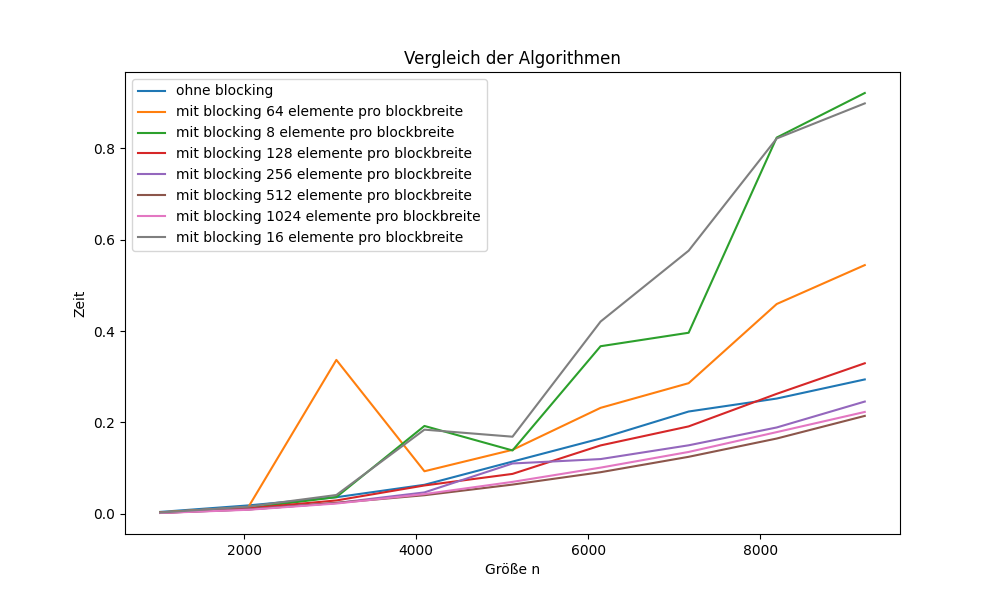
\includegraphics[width=0.525\textwidth]{blocking_MVP.png}
    \label{MVPblocked}
\end{figure}


\begin{tiny}
    \begin{adjustwidth}{-0,37cm}{}
    \begin{footnotesize}
    \begin{auflistung}
    \caption{Implementierung der blockierten Matrixtransposition}
    \label{Matrixtransposition}
    \begin{minted}[linenos, gobble=2,xleftmargin=-0.3cm, numbersep=-12pt]{cpp}
        transpose_blocked(double *A, double *B, int n, size_t blockSize)
        {
            if(blockSize > n){
                blockSize = n;
            } 
            size_t nBlocks = n / blockSize;
            for (size_t i_block = 0; i_block < nBlocks; i_block++)
            {
            for (size_t j_block = 0; j_block < nBlocks; j_block++)
            {
            for (size_t i = i_block * blockSize; i < (i_block + 1) * blockSize; i++)
            {
            for (size_t j = j_block * blockSize; j < (j_block + 1) * blockSize; j++)
            {
                B[i * n + j] = A[j * n + i];
            }
            }
            }
            }
        }
\end{minted}
\end{auflistung}
\end{footnotesize}
\end{adjustwidth}
\end{tiny}

Blocking ist eine Methode, 
bei der die Problemgröße in kleinere Teile aufgeteilt und diese nacheinander bearbeitet werden. 
Dies kann dazu beitragen, die zeitliche Lokalität zu verbessern, 
da kontinuierlich auf dieselben Daten zugegriffen wird. 
Bei der Unroll-and-Jam-Implementierung zur Transposition einer Matrix konnte die Bandbreite erhöht werden, 
indem statt eines Elements fünf Elemente einer Cachezeile genutzt wurden, 
bevor diese verdrängt wurde. Blocking kann nun dazu beitragen, 
zusätzlich zu den fünf Elementen auch die restlichen Elemente der Cachezeile zu nutzen, 
bevor diese verdrängt wird. Der beste Weg herauszufinden welche Blockgröße die beste ist,
ist es die Implementierung mit verschiedenen Blockgrößen zu testen und die Bandbreite zu messen.
In der Abbildung \ref{MVPblocked} ist die Bandbreite für verschiedene Blockgrößen dargestellt.
Es hat sich herausgestellt, dass eine Blockgröße von 512 auf dem i7-9700K beispielsweise bei dem Matrix Vektor Produkt am wenigsten Zeit benötigte,
von den blocking-Werten die getestet wurden. Die "Größe n" gibt die Dimensionsgrößen der Matrix und der Vektoren an das heißt:
$A \in \mathbb{R}^{m \times n}$, $C \in \mathbb{R}^{n \times 1}$, $B \in \mathbb{R}^{n \times 1}$. Für alle $\textnormal{n}$, berechnet man:
$C^{n\times 1} += A^{n \times n} \cdot B^{n \times 1}$.


Blocking kann man auch auf das Transponieren einer Matrix anwenden. 
In Auflistung \ref{Matrixtransposition} ist eine Implementierung der blockierten Matrixtransposition dargestellt.
Die Matrix wird in kleinere Blöcke aufgeteilt und diese Blöcke werden nacheinander transponiert, wobei man jetzt
nur den Fall betrachtet bei dem die Matrix quadratisch ist, 
die Blockgröße ein Teiler der Matrixgröße ist.






\section{Fazit}








%%
%% The acknowledgments section is defined using the "acks" environment
%% (and NOT an unnumbered section). This ensures the proper
%% identification of the section in the article metadata, and the
%% consistent spelling of the heading.
%\begin{acks}

%\end{acks}

%%
%% The next two lines define the bibliography style to be used, and
%% the bibliography file.


%%\begin{figure}[H]
%%    \caption{\textbf{Basistaktfrequenzen von Intel Prozessoren} (Datenquelle: \cite{Comparison})}
  %%  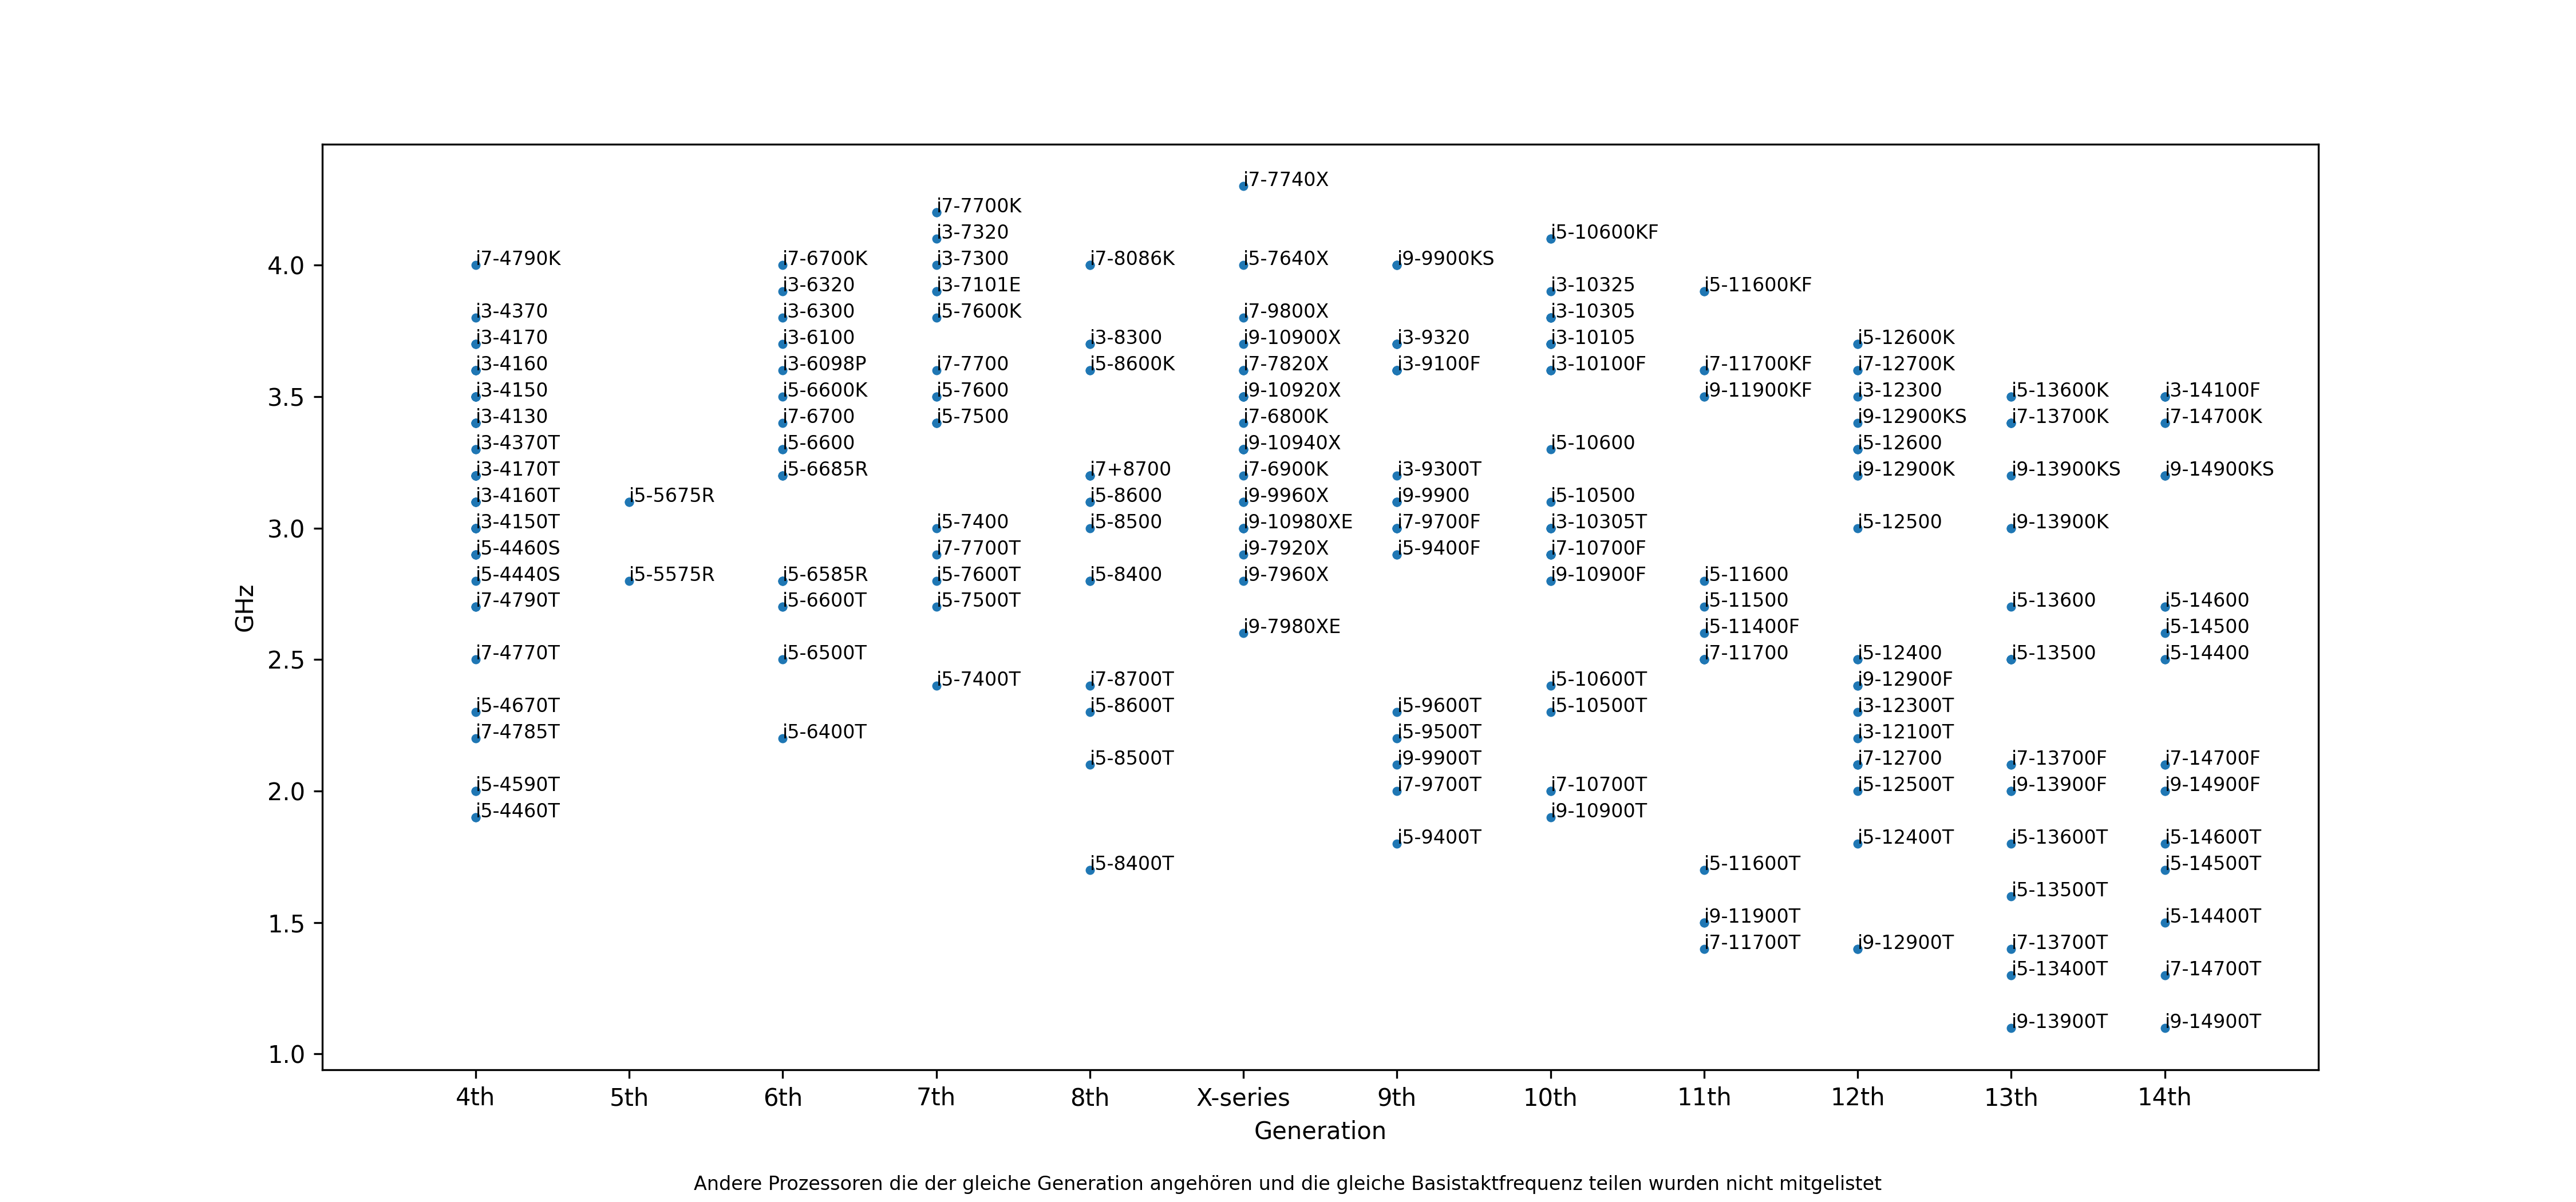
\includegraphics[width=0.99\textwidth]{Abbildung_last.png}
  %%  \label{fig:Abbildung_last} 
  %%  \end{figure}


\bibliographystyle{ACM-Reference-Format}
\bibliography{sample-base}


%%
%% If your work has an appendix, this is the place to put it.
\appendix



\end{document}
\endinput
%%
%% End of file `sample-acmtog.tex'.
